\begin{table}[h]
	\begin{tabular}{lll}
		\hline
		\textbf{Constraints}& \textbf{string representation}\\
		\hline
		\textbf{\textsc{*LH}$_\sigma$}    & *LH \\
		\textbf{\textsc{*Contour}$_{\mu}$} & *R, *F\\
		\textbf{\textsc{*3t-Contour}}&*HLL,*HHH,*LLL\\
		\textbf{\textsc{*Clash}}& *LL\\
		\textbf{\textsc{*NonfinalHL}}& *HL.\\
		\hline
	\end{tabular}\caption{}
	\label{rules}
\end{table}


\begin{table}
	%		\centering
	\begin{tabular}{c}
		\hline
		
		\scalebox{0.7}{\begin{subfigure}[t]{1.5cm}
				\centering
				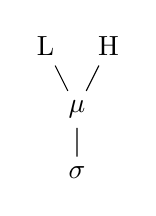
\begin{tikzpicture}
					\node (bt1) at (-.4,0.8) {L};
					\node (bt2) at (.4,0.8) {H};
					\node (bc1) at (0,0) {$\mu$};
					\node (bs1) at (0,-0.8) {$\sigma$};
					\draw (bt1) -- (bc1) -- (bs1);
					\draw (bt2) -- (bc1);
				\end{tikzpicture}
				\vspace{-0.5em}
				\subcaption{}
		\end{subfigure}} 
		
		\scalebox{0.7}{\begin{subfigure}[t]{1.5cm}			
				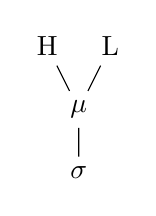
\begin{tikzpicture}
					\node (bt1) at (-.4,0.8) {H};
					\node (bt2) at (.4,0.8) {L};
					\node (bc1) at (0,0) {$\mu$};
					\node (bs1) at (0,-0.8) {$\sigma$};
					\draw (bt1) -- (bc1) -- (bs1);
					\draw (bt2) -- (bc1);
				\end{tikzpicture}
				\vspace{-0.5em}
				\subcaption{}
		\end{subfigure}} 
		
		\scalebox{0.7}{			\begin{subfigure}[t]{1.5cm}
				\centering 
				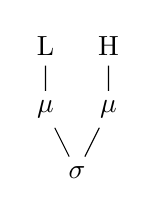
\begin{tikzpicture}
					\node (bt1) at (-.4,0.8) {L};
					\node (bt2) at (.4,0.8) {H};
					\node (bc1) at (-.4,0) {$\mu$};
					\node (bc2) at (.4,0) {$\mu$};
					\node (bs1) at (0,-0.8) {$\sigma$};
					\draw (bt1) -- (bc1) -- (bs1);
					\draw (bt2) -- (bc2) -- (bs1);
				\end{tikzpicture}
				\vspace{-0.5em}
				\subcaption{}
		\end{subfigure}} 
		%				\hspace{-1.3em}
		\scalebox{0.7}{			\begin{subfigure}[t]{1.6cm}
				\vspace{-4em}
				\centering				
				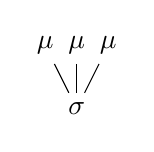
\begin{tikzpicture}
					\node (bc1) at (-.4,0) {$\mu$};
					\node (bc2) at (0,0) {$\mu$};
					\node (bc3) at (.4,0) {$\mu$};
					\node (bs1) at (0,-0.8) {$\sigma$};
					\draw (bc1) -- (bs1);
					\draw (bc2) -- (bs1);
					\draw (bc3) -- (bs1);
				\end{tikzpicture}
				\vspace{0.2em}
				\subcaption{}
		\end{subfigure}} 
		
		\scalebox{0.7}{	\begin{subfigure}[t]{1.6cm}
				\centering
				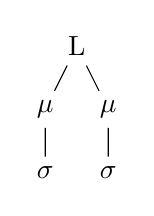
\begin{tikzpicture}
					\node (bt1) at (0,0.8) {L};
					% \node (bt2) at (.4,0.8) {L};
					\node (bc1) at (-.4,0) {$\mu$};
					\node (bc2) at (.4,0) {$\mu$};
					\node (bs1) at (-.4,-0.8) {$\sigma$};
					\node (bs2) at (0.4,-0.8) {$\sigma$};
					\draw (bt1) -- (bc1) -- (bs1);
					\draw (bt1) -- (bc2) -- (bs2);
				\end{tikzpicture}
				\vspace{-0.5em}
				\subcaption{}
		\end{subfigure}} 
		
		\scalebox{0.7}{			\begin{subfigure}[t]{2cm}
				\centering
				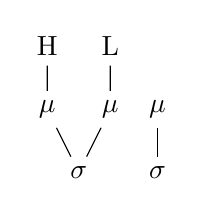
\begin{tikzpicture}
					\node (bt1) at (-.4,0.8) {H};
					\node (bt2) at (.4,0.8) {L};
					\node (bc1) at (-.4,0) {$\mu$};
					\node (bc3) at (1,0) {$\mu$};
					\node (bc2) at (.4,0) {$\mu$};
					\node (bs1) at (0,-0.8) {$\sigma$};
					\node (bs2) at (1,-0.8) {$\sigma$};
					\draw (bt1) -- (bc1) -- (bs1);
					\draw (bt2) -- (bc2) -- (bs1);
					\draw (bc3) -- (bs2);
				\end{tikzpicture}				\vspace{-.5em}
				\subcaption{}
		\end{subfigure}} \\ \hline
	\end{tabular} \caption{}
	\label{rules}
\end{table}